\documentclass[10pt,a4paper]{article}
\usepackage{graphicx}
\usepackage{booktabs}
\setlength{\textwidth}{165mm}\setlength{\oddsidemargin}{-2mm}
\setlength{\textheight}{245mm}\setlength{\topmargin}{-13mm}
\setlength{\parindent}{0pt}\setlength{\parskip}{4pt}
\tolerance=2000\setlength{\emergencystretch}{3em}

\title{Automatic Selection of Temporal Features for Music Recommendation}
\author{Vladislav Neklydov}\date{25 October 2026}
\begin{document}\maketitle


\begin{abstract}
We evaluate automatic group selection over a temporal feature dictionary
against a fixed manual gradient-boosting baseline on a 1,000-user Yambda cohort.
Selection uses an earlier development slice; a later development slice and
a subsequently frozen temporal holdout are reported separately.
On the frozen P20 holdout the automatic-minus-manual NDCG difference is +0.000567 [-0.000550, +0.001672] (paired 95\% user-cluster interval).
The comparison includes a full-dictionary control, matched hard-window and
decay features, paired uncertainty estimates and computational costs.
\end{abstract}
\section{Introduction}
Manual recommendation features require choices about relations, aggregation
and time scales. We study whether automatic selection of temporal feature
groups can preserve ranking quality relative to a manual gradient-boosting
baseline. Candidate groups combine user, item and user--item histories at
prespecified time scales. The learner, data and candidate protocol are held
fixed across representations.

Earlier development experiments informed the research design. Feature selection
uses an earlier validation interval; a later validation interval and a
subsequently frozen temporal test are evaluated separately. Test data are not
used for feature selection or model refitting.

\section{Data and task}
We use the pinned Yambda 50m multi-event release [1], with its raw size and
SHA256 recorded in the repository. The 1,000-user cohort retains an initial 100-user development sample and
adds 900 deterministically sampled users. Complete release histories are retained. Query caps limit
training/evaluation targets, not the histories used to construct features.
The task ranks a logged listen among twenty distinct alternatives. Alternatives
are unobserved candidates, not verified dislikes or non-clicked impressions.
This is sampled positive-target ranking, not a full-catalog or CTR benchmark.

Recorded timestamps are seconds, quantized to five seconds. Training ends
exclusively at 20,800,000; development ends at 23,400,000. The final interval
is [23,400,000, 26,000,000]. A 30,000-query training cap and 20,000-query caps
for development and holdout are fixed. Observed counts appear below.
\clearpage
\section{Information boundary and comparable models}
Every feature at time $t$ uses only recorded events with $s<t$; all equal-time
events and the target itself are excluded. Candidates come from the
training-defined catalog and must have appeared strictly before $t$.
Targets with ambiguous user/timestamp groups, insufficient prior history,
training-ineligible users or out-of-catalog items are excluded identically
across representations. Novel targets have no earlier user--item interaction;
they need not be globally new items. These exclusions restrict generalization.

U20 samples alternatives uniformly. P20 samples sequentially without replacement
with weights $c_i(t)+1$, using strictly prior counts in the retained cohort.
Targets match across protocols, while candidates and protocol-specific training
examples differ. Within each protocol every representation uses identical
queries/candidates. Cross-protocol score differences are not model gains.

The pointwise histogram gradient-boosting classifier has learning rate 0.08,
80 iterations, at most 15 leaves, depth 4, minimum leaf size 30, $L_2=1$,
no early stopping, and seed 20261024. The same learner fits every feature set.
The original representation has 9 features; its no-pair ablation has 6.
The stronger manual representation has 17: cumulative counts/recencies and
7/30-day user, item and pair windows, with smoothed shares/affinities.
Matched decay features replace the windows by exponential half-lives.
The full dictionary has 47 columns over 1/7/30/90-day scales.

For the prior events $H_R(t)$ matching a user, item or pair relation,
the hard count is $C_h(t)=\sum_{s\in H_R(t)}\mathbf{1}\{t-h\leq s<t\}$;
the matched decay count is $D_h(t)=\sum_{s\in H_R(t)}2^{-(t-s)/h}$.
Smoothed affinities include $(D_h^{\rm pair}+1)/(D_h^{\rm user}+2)$.
Counts include all recorded event types; they measure interaction, not
uniformly positive preference. Histories start at the released data boundary.

\section{Automatic procedure and evaluation discipline}
Start from the 17 manual features. Six declared groups add extra hard windows
or decay features for user, item and pair relations. Fit each of the six
one-group additions on the same training data. Rank candidates by P20
event NDCG@10 on V\_search (timestamps before 22,100,000), with a fixed
minimum gain of 0.0001. Retain the manual baseline if no candidate clears
that threshold. The bounded configuration uses one forward round and an
eight-fit cap. It is automated selection within a human-designed grammar.

The automatic procedure selected user\_item\_decay\_all, giving 25 features. It adds four pair-decay counts and four smoothed pair/user decay affinities at 1/7/30/90-day half-lives; it does not learn an unrestricted window length.
Both searches cover the same six one-group additions in different orders. Their agreement is expected under this exhaustive one-round comparison; it does not distinguish optimizer quality.
The later V\_check slice is not used by this procedure to select features.
It is still reused development evidence, not a pristine test. U20 applies the
P20-selected feature list without performing another feature search.

Feature sets, fitted models, sampling rules and comparisons are fixed before
test scoring. All models retain their training-only fits; there is no refitting
on validation data or optimization on the test interval.
Online histories may include earlier holdout events, which would already be
recorded at the prediction time. This prequential information policy is
shared by all methods and differs from freezing every history at the split.
\clearpage
\section{Quality and uncertainty}
The main development panel has 20,000 queries from 744 evaluated users. The holdout has 20,000 queries from 772 users, including 4,604 novel-target queries. Eligible evaluated-user counts are reported separately for each interval.
Table columns Search/Check show event NDCG@10 on the two development slices;
Test shows event NDCG@10 on the frozen holdout. Recall is test Recall@10.
\subsection*{P20: popularity-weighted alternatives}\begin{center}\small\begin{tabular}{lrrrrr}\toprule Method & Features & Search & Check & Test & Recall\\\midrule
Original & 9 & 0.797828 & 0.787039 & 0.773804 & 0.903050 \\
No pair & 6 & 0.407213 & 0.384224 & 0.378794 & 0.677550 \\
Manual & 17 & 0.804505 & 0.790649 & 0.778141 & 0.903850 \\
Decay & 17 & 0.804314 & 0.791068 & 0.778764 & 0.906400 \\
All features & 47 & 0.803637 & 0.790897 & 0.778828 & 0.906550 \\
Automatic & 25 & 0.804830 & 0.790544 & 0.778708 & 0.903250 \\
Matched search & 25 & 0.804830 & 0.790544 & 0.778708 & 0.903250 \\\bottomrule\end{tabular}\end{center}\subsection*{U20: uniform alternatives}\begin{center}\small\begin{tabular}{lrrrrr}\toprule Method & Features & Search & Check & Test & Recall\\\midrule
Original & 9 & 0.918904 & 0.909705 & 0.905634 & 0.982350 \\
No pair & 6 & 0.761738 & 0.748490 & 0.748303 & 0.968700 \\
Manual & 17 & 0.920079 & 0.910035 & 0.907320 & 0.983000 \\
Decay & 17 & 0.920256 & 0.910038 & 0.907150 & 0.982150 \\
All features & 47 & 0.920338 & 0.909885 & 0.907373 & 0.982700 \\
Automatic & 25 & 0.920526 & 0.910350 & 0.907610 & 0.983250 \\
Matched search & 25 & 0.920526 & 0.910350 & 0.907610 & 0.983250 \\\bottomrule\end{tabular}\end{center}

\begin{center}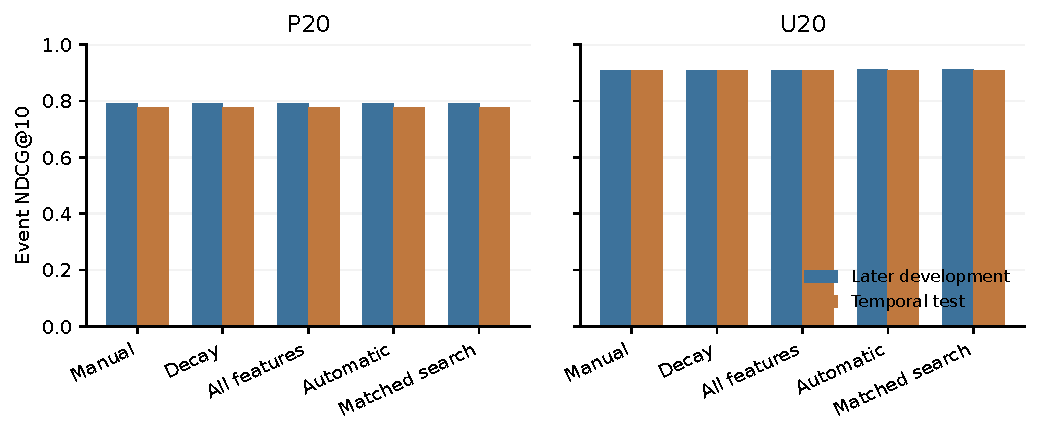
\includegraphics[width=\linewidth,height=66mm,keepaspectratio]{quality.pdf}\end{center}
NDCG@10 equals $\mathbf{1}\{r\leq10\}/\log_2(r+1)$ and Recall@10 equals
$\mathbf{1}\{r\leq10\}$ for positive rank $r$. Ties use deterministic
label-independent keys. Event weighting is primary, with repeat and novel
targets analyzed separately. Paired percentile intervals
resample users 1,000 times, retaining their queries and candidate pairing.
They condition on the observed cohort, interval and sampling design; they do
not account for adaptive question formation or exploratory multiplicity.
\clearpage
\section{What automation changed}
On the final P20 interval, automatic minus manual NDCG@10 is
+0.000567 [-0.000550, +0.001672].

The 0.005 tolerance is a study-specific practical criterion, not an established application threshold. The interval spans zero: these data do not establish a gain or loss in event-average ranking. Its lower endpoint exceeds the chosen -0.005 tolerance, supporting that limited tolerance claim here. A gain of 0.005 is outside the reported interval.

The full-dictionary control assesses whether using every available feature
improves on the manual baseline.
Matched decays isolate temporal shape at approximately matched feature count.
\begin{center}\small\begin{tabular}{llrrr}\toprule Slice & Difference & Estimate & Lower & Upper\\\midrule
Check & forward - manual & -0.000104 & -0.001780 & +0.001558 \\
Check & all - manual & +0.000249 & -0.001581 & +0.002073 \\
Check & decay - manual & +0.000419 & -0.001526 & +0.002402 \\
Test & forward - manual & +0.000567 & -0.000550 & +0.001672 \\
Test & all - manual & +0.000687 & -0.000617 & +0.002121 \\
Test & decay - manual & +0.000623 & -0.000788 & +0.002082 \\\bottomrule\end{tabular}\end{center}

\begin{center}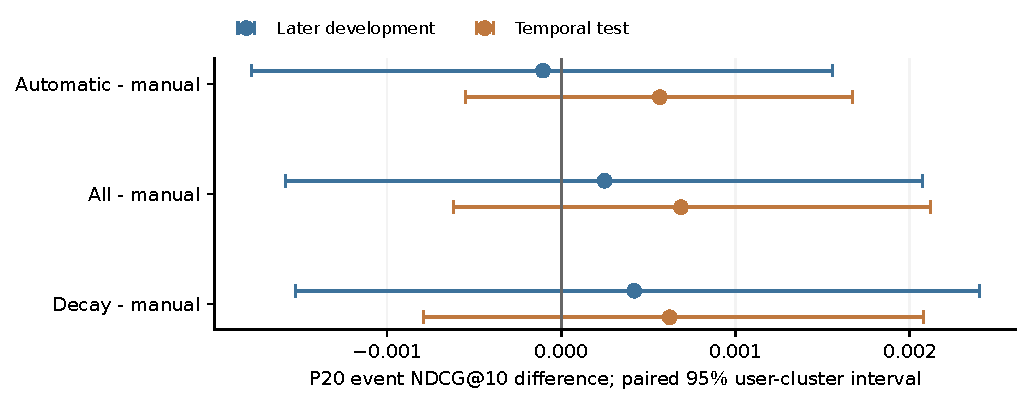
\includegraphics[width=\linewidth,height=66mm,keepaspectratio]{effects.pdf}\end{center}
\begin{center}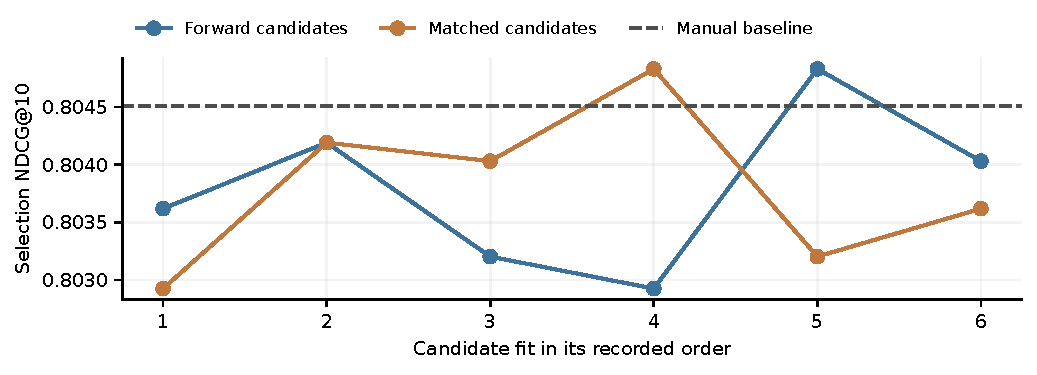
\includegraphics[width=\linewidth,height=53mm,keepaspectratio]{search.pdf}\end{center}
The search trace is a selection diagnostic. Its best score must not be
reported as an unbiased estimate of out-of-selection performance.
\clearpage
\section{Diagnostic ablation and computation}
\begin{center}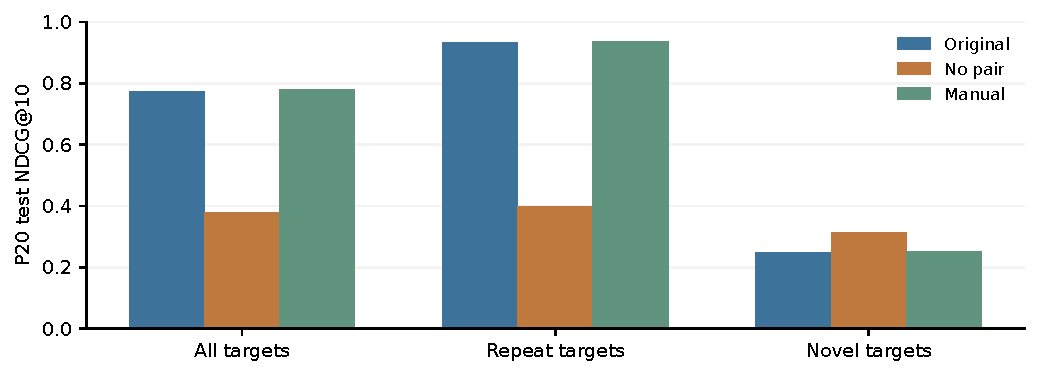
\includegraphics[width=\linewidth,height=68mm,keepaspectratio]{repetition.pdf}\end{center}
On P20 test data, no-pair-minus-original is -0.395010 [-0.407967, -0.383487] overall and +0.066338 [+0.052535, +0.078552] on novel targets. All intervals here use event weighting.
Aggregate quality alone can therefore conceal a repeat/novel tradeoff.
It does not follow that removing pair features is a good overall replacement.

\begin{center}\small\begin{tabular}{lrrr}\toprule Method & Job wall (s) & Fit(s) & Tree RSS (GiB)\\\midrule
Manual & 6.544 & 2.182 & 0.876 \\
All features & 8.812 & 4.222 & 1.078 \\
Automatic & 23.110 & 14.468 & 0.945 \\
Matched search & 24.636 & 15.680 & 0.946 \\\bottomrule\end{tabular}\end{center}

Timings were measured on Linux x86\_64 with four worker threads. Job wall time includes process startup and recorded work. Fit time is one
fixed-model fit or the sum of candidate fits for search; it is not total
pipeline cost. Imports, feature materialization, inference and serialization
have different boundaries. Identical fitted finalists may be reused within
the native immutable run, with reuse explicitly recorded.
The full 47-column dictionary is materialized even for compact feature sets.
Fewer selected columns do not establish cheaper feature construction.
RSS is a sampled process-tree sum; shared pages can be counted twice and
short spikes missed. These are observed local costs, not a validated
scaling law.

\section{Limitations and conclusions}
This is one bounded, development-adaptive study with a fixed learner, finite
cohort and sampled candidates. It does not model exposure or validate
ingestion-time availability. Training-catalog/user eligibility excludes cold
targets. Bootstrap intervals do not establish robustness to another time
period, cohort, hyperparameter setting or full-catalog evaluation.
The automatic grammar omits artist/category relations and unrestricted
new aggregation synthesis. One-step enumeration is intentionally small.
The result supports only the methods, information boundary and population
actually evaluated. Further work should vary the cohort and time period
after preserving this holdout result, and compare stronger relational
grammars under explicit search and feature-construction budgets.
\clearpage
\section{Relation to prior work}
Deep Feature Synthesis follows relational paths and composes transformations
to generate predictive features [2]. Our grammar is much narrower: known
user/item/pair histories and temporal aggregations. Khurana et al. automate
performance-driven exploration of a transformation graph with a learned
reinforcement-learning strategy [3]. We implement neither that learned
policy nor unrestricted transformation search; our small enumeration makes
the available search space and budget easy to audit. Yambda's authors provide
a music-interaction dataset and global temporal evaluation protocol [1].
Our selected release/cohort and sampled positive-target task are explicitly
different from a reproduction of their full benchmark.

\begin{thebibliography}{9}
\bibitem{yambda} A. Ploshkin et al. Yambda-5B: A Large-Scale Multi-modal
Dataset for Ranking and Retrieval. arXiv:2505.22238, 2025.
\bibitem{dfs} J. M. Kanter and K. Veeramachaneni. Deep Feature Synthesis:
Towards Automating Data Science Endeavors. IEEE DSAA, 2015.
\bibitem{rl} U. Khurana, H. Samulowitz and D. Turaga. Feature Engineering
for Predictive Modeling Using Reinforcement Learning. AAAI, 2018.
\end{thebibliography}

\end{document}
